\documentclass[border=12pt]{standalone}
\usepackage{tikz}
\usetikzlibrary{calc,intersections,through}

\begin{document}
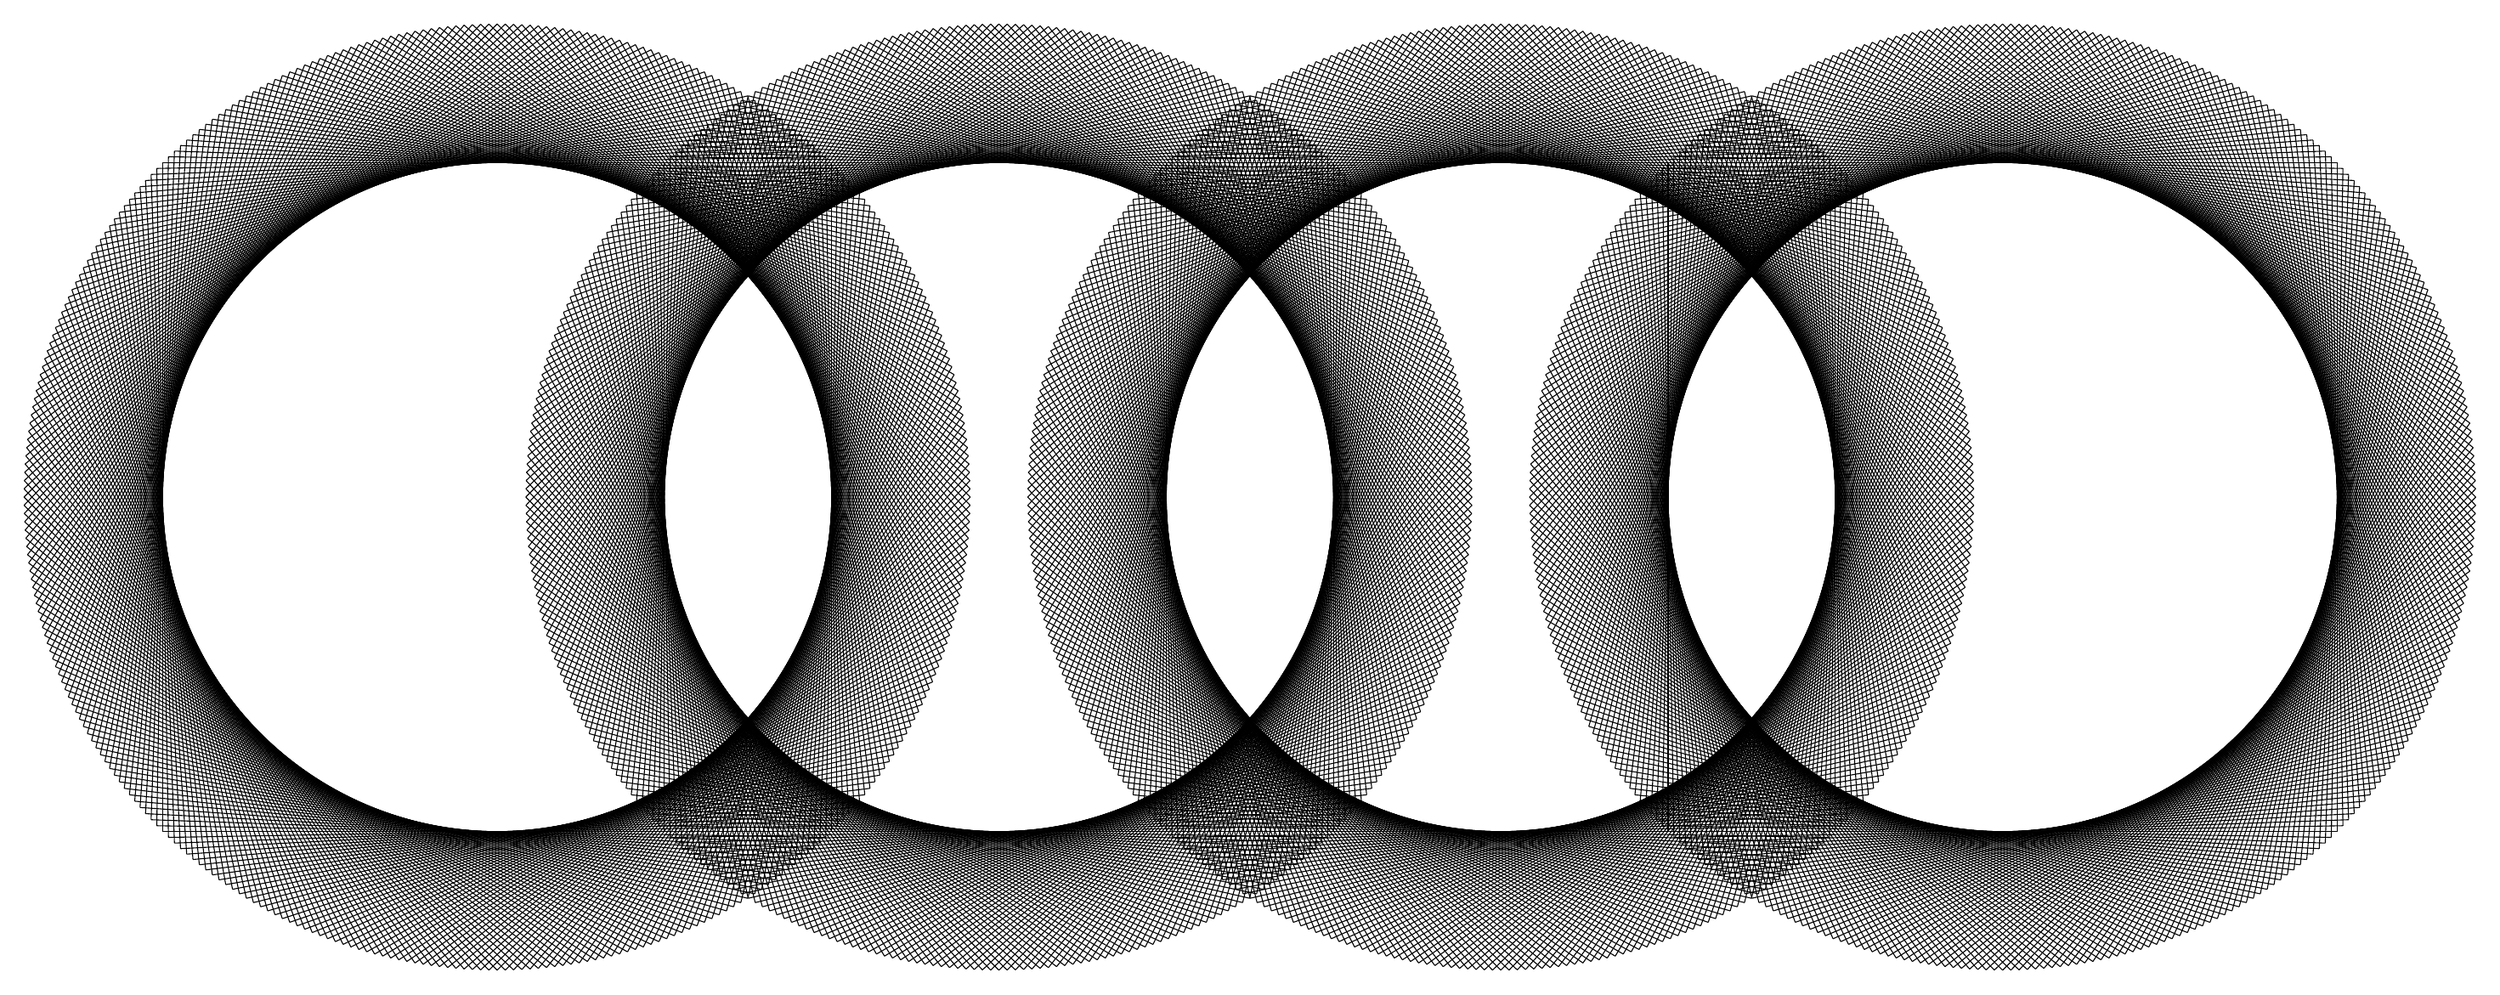
\begin{tikzpicture}

% rotate=\deg与rotate around={\deg:(0,0)}]等效
\foreach \deg in {0,...,359} {
	\draw [rotate around={\deg:(0,0)}] (5,5) -- ++(-10,0);
	\draw [rotate around={\deg:(7.5,0)}] (12.5,5) -- ++(-10,0);
	\draw [rotate around={\deg:(15,0)}] (20,5) -- ++(-10,0);
	\draw [rotate around={\deg:(22.5,0)}] (27.5,5) -- ++(-10,0);
}

%\fill (0,0) coordinate (O) circle[radius=1pt] node[below] {$O$};
%\fill (5,5) coordinate (O') circle[radius=1pt] node[below] {$O'$};
%\fill (-5,5) coordinate (O'') circle[radius=1pt] node[below] {$O''$};
%\draw (O) -- (O');
%\draw (O) -- (O'');

\end{tikzpicture}
\end{document}
